\documentclass[border=3pt,tikz]{standalone}
\usepackage{amsmath,amssymb,amsfonts}
\usepackage{tikz}
\usetikzlibrary{shapes,arrows.meta,positioning,calc,decorations.pathreplacing,decorations.markings,patterns,backgrounds,shadows,fit}

% Academic Color Palette (IEEE Standard Muted Tones)
\definecolor{primaryblue}{RGB}{20, 45, 85}
\definecolor{accentblue}{RGB}{35, 85, 140}
\definecolor{safegreen}{RGB}{38, 115, 50}
\definecolor{safegreenbg}{RGB}{236, 246, 238}
\definecolor{safegreenborder}{RGB}{140, 200, 150}
\definecolor{dangerred}{RGB}{190, 35, 35}
\definecolor{dangerredbg}{RGB}{254, 237, 238}
\definecolor{dangerredborder}{RGB}{240, 160, 160}
\definecolor{warnorange}{RGB}{215, 100, 0}
\definecolor{warnyellowbg}{RGB}{255, 250, 235}
\definecolor{warnyellowborder}{RGB}{250, 210, 140}
\definecolor{tieorangebg}{RGB}{255, 242, 225}
\definecolor{tieorangeborder}{RGB}{250, 190, 120}
\definecolor{backupcolor}{RGB}{110, 35, 150}
\definecolor{backupbg}{RGB}{246, 238, 250}
\definecolor{panelbg}{RGB}{252, 253, 254}
\definecolor{panelborder}{RGB}{210, 218, 228}
\definecolor{darkslate}{RGB}{45, 55, 65}
\definecolor{midgray}{RGB}{125, 138, 150}

\begin{document}
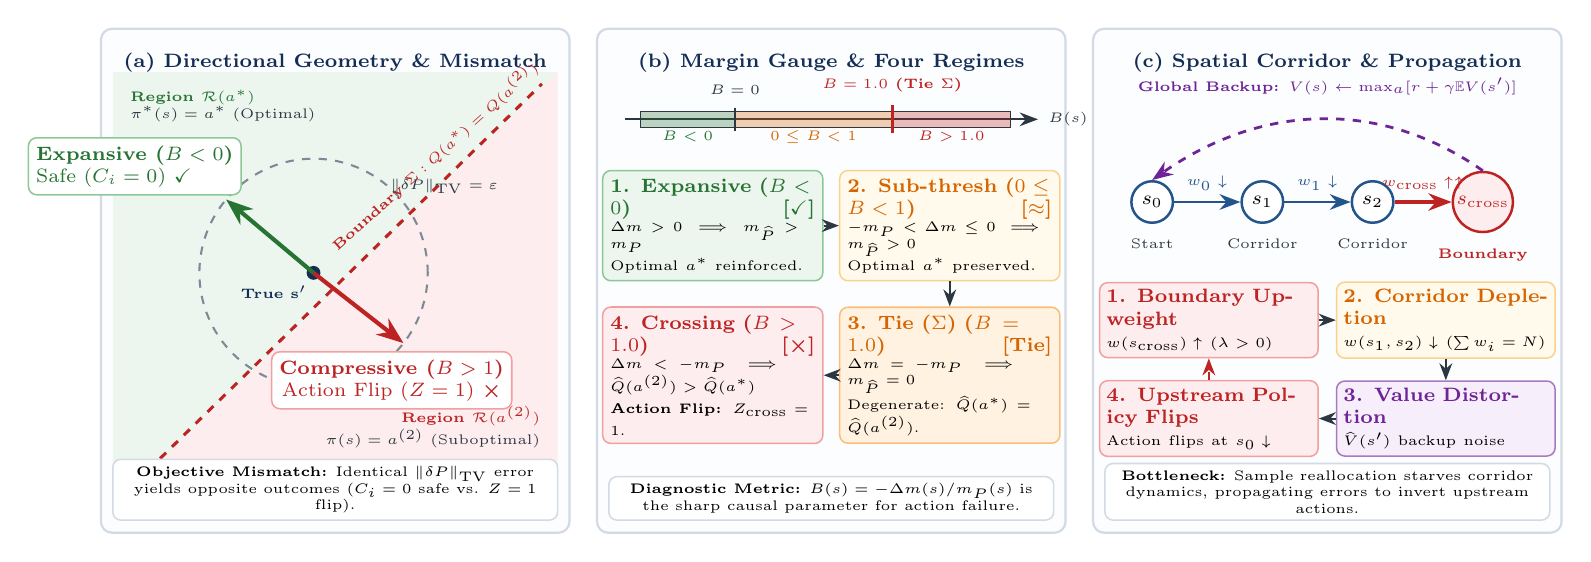
\begin{tikzpicture}[
    font=\small,
    >=Stealth,
    panel/.style={
        draw=panelborder,
        fill=panelbg,
        rounded corners=4pt,
        line width=0.8pt
    },
    boxcard/.style={
        rounded corners=3pt,
        line width=0.55pt,
        inner sep=2.8pt,
        font=\scriptsize
    },
    state/.style={
        circle,
        draw=accentblue,
        fill=white,
        line width=0.9pt,
        minimum size=15pt,
        inner sep=1pt,
        font=\scriptsize\bfseries
    }
]

% Panel Dimensions & Grid Layout (Compact Gold Standard: 6.4cm Height)
\def\PW{5.95}  % Panel Width
\def\PH{6.4}   % Panel Height (~20% of IEEE journal page)
\def\GAP{0.35} % Gap between panels

% ==============================================================================
% PANEL (A): DIRECTIONAL GEOMETRY & OBJECTIVE MISMATCH
% ==============================================================================
\begin{scope}[shift={(0,0)}]
    \draw[panel] (0,0) rectangle (\PW, \PH);
    \node[font=\bfseries\scriptsize, text=primaryblue, anchor=north] at (\PW/2, \PH-0.18) {(a) Directional Geometry \& Mismatch};

    \coordinate (O) at (2.7, 3.3);
    
    % Clip boundary for geometric regions
    \begin{scope}
        \clip (0.15, 0.85) rectangle (\PW-0.15, \PH-0.55);
        \fill[safegreenbg] (0.15, 0.85) -- (0.15, \PH-0.55) -- (\PW-0.15, \PH-0.55) -- (0.7, 0.85) -- cycle;
        \fill[dangerredbg] (0.7, 0.85) -- (\PW-0.15, \PH-0.55) -- (\PW-0.15, 0.85) -- cycle;
        \draw[dangerred, dashed, line width=1.1pt] (0.3, 0.5) -- (5.6, 5.7);
        \draw[midgray, dashed, line width=0.75pt] (O) circle (1.45cm);
    \end{scope}

    \node[font=\tiny\bfseries, text=dangerred, rotate=42, anchor=south] at (4.4, 4.6) {Boundary $\Sigma: Q(a^*) = Q(a^{(2)})$};
    \node[font=\tiny\itshape, text=darkslate, anchor=west] at ($(O)+(0.85, 1.1)$) {$\|\delta P\|_{\mathrm{TV}} = \varepsilon$};

    % Region Labels
    \node[anchor=north west, align=left, font=\tiny] at (0.25, \PH-0.65) {
        \textcolor{safegreen}{\textbf{Region $\mathcal{R}(a^*)$}}\\
        \textcolor{darkslate}{$\pi^*(s) = a^*$ (Optimal)}
    };
    \node[anchor=south east, align=right, font=\tiny] at (\PW-0.25, 0.95) {
        \textcolor{dangerred}{\textbf{Region $\mathcal{R}(a^{(2)})$}}\\
        \textcolor{darkslate}{$\pi(s) = a^{(2)}$ (Suboptimal)}
    };

    % Nominal State Dot
    \fill[primaryblue] (O) circle (2.5pt) node[anchor=north east, font=\tiny\bfseries, text=primaryblue, yshift=-1pt, xshift=1pt] {True $\mathbf{s}'$};

    % Expansive Error Vector
    \draw[->, safegreen, line width=1.5pt] (O) -- ++(140:1.45) coordinate (EXP_END);
    \node[boxcard, fill=white, draw=safegreenborder, text=safegreen, anchor=south east, align=left] at ($(EXP_END)+(0.2, 0.05)$) {
        \textbf{Expansive ($B < 0$)}\\Safe ($C_i = 0$) $\checkmark$
    };

    % Compressive Error Vector
    \draw[->, dangerred, line width=1.5pt] (O) -- ++(-38:1.45) coordinate (COMP_END);
    \node[boxcard, fill=white, draw=dangerredborder, text=dangerred, anchor=north, align=center] at ($(COMP_END)+(-0.15, -0.1)$) {
        \textbf{Compressive ($B > 1$)}\\Action Flip ($Z=1$) $\boldsymbol{\times}$
    };

    % Bottom Takeaway Box
    \node[boxcard, fill=white, draw=panelborder, anchor=south, minimum width=\PW cm - 0.3cm, inner sep=2.5pt] at (\PW/2, 0.15) {
        \parbox{5.4cm}{\centering \tiny \textbf{Objective Mismatch:} Identical $\|\delta P\|_{\mathrm{TV}}$ error yields opposite outcomes ($C_i = 0$ safe vs. $Z = 1$ flip).}
    };
\end{scope}

% ==============================================================================
% PANEL (B): DECISION MARGIN GAUGE & 2x2 REGIME MATRIX (Clockwise Flow 1->2->3->4)
% ==============================================================================
\begin{scope}[shift={(\PW+\GAP, 0)}]
    \draw[panel] (0,0) rectangle (\PW, \PH);
    \node[font=\bfseries\scriptsize, text=primaryblue, anchor=north] at (\PW/2, \PH-0.18) {(b) Margin Gauge \& Four Regimes};

    % Top 1D Pressure Spectrum Gauge
    \def\GY{5.25}
    \draw[->, line width=0.8pt, darkslate] (0.35, \GY) -- (\PW-0.35, \GY) node[anchor=west, font=\tiny\bfseries] {$B(s)$};
    
    \fill[safegreen, opacity=0.3] (0.55, \GY-0.1) rectangle (1.75, \GY+0.1);
    \fill[warnorange, opacity=0.3] (1.75, \GY-0.1) rectangle (3.75, \GY+0.1);
    \fill[dangerred, opacity=0.3] (3.75, \GY-0.1) rectangle (5.25, \GY+0.1);
    \draw[line width=0.4pt, darkslate] (0.55, \GY-0.1) rectangle (5.25, \GY+0.1);

    \draw[line width=0.8pt, darkslate] (1.75, \GY-0.15) -- (1.75, \GY+0.15) node[above=1pt, font=\tiny\bfseries] {$B=0$};
    \draw[line width=1.0pt, dangerred] (3.75, \GY-0.18) -- (3.75, \GY+0.18) node[above=1pt, font=\tiny\bfseries, text=dangerred] {$B=1.0$ (Tie $\Sigma$)};

    \node[font=\tiny\bfseries, text=safegreen] at (1.15, \GY-0.22) {$B<0$};
    \node[font=\tiny\bfseries, text=warnorange] at (2.75, \GY-0.22) {$0\le B<1$};
    \node[font=\tiny\bfseries, text=dangerred] at (4.5, \GY-0.22) {$B>1.0$};

    % 2x2 Matrix of Regime Cards in Clockwise Harmonic Flow
    \def\CW{2.74cm}
    
    % Regime 1 (Top Left)
    \node[boxcard, fill=safegreenbg, draw=safegreenborder, minimum width=\CW, text width=2.6cm, align=left] (R1) at (1.47, 3.9) {
        \textcolor{safegreen}{\textbf{1. Expansive ($B < 0$)}}\hfill\textcolor{safegreen}{\textbf{[$\checkmark$]}}\\
        \tiny $\Delta m > 0 \implies m_{\widehat{P}} > m_P$\\
        Optimal $a^*$ reinforced.
    };

    % Regime 2 (Top Right)
    \node[boxcard, fill=warnyellowbg, draw=warnyellowborder, minimum width=\CW, text width=2.6cm, align=left] (R2) at (4.48, 3.9) {
        \textcolor{warnorange}{\textbf{2. Sub-thresh ($0\le B<1$)}}\hfill\textcolor{warnorange}{\textbf{[$\approx$]}}\\
        \tiny $-m_P < \Delta m \le 0 \implies m_{\widehat{P}} > 0$\\
        Optimal $a^*$ preserved.
    };

    % Regime 3 (Bottom Right - Natural Clockwise step from 2)
    \node[boxcard, fill=tieorangebg, draw=tieorangeborder, minimum width=\CW, text width=2.6cm, align=left] (R3) at (4.48, 2.0) {
        \textcolor{warnorange}{\textbf{3. Tie ($\Sigma$) ($B=1.0$)}}\hfill\textcolor{warnorange}{\textbf{[Tie]}}\\
        \tiny $\Delta m = -m_P \implies m_{\widehat{P}} = 0$\\
        Degenerate: $\widehat{Q}(a^*) = \widehat{Q}(a^{(2)})$.
    };

    % Regime 4 (Bottom Left - Final Failure Endpoint)
    \node[boxcard, fill=dangerredbg, draw=dangerredborder, minimum width=\CW, text width=2.6cm, align=left] (R4) at (1.47, 2.0) {
        \textcolor{dangerred}{\textbf{4. Crossing ($B>1.0$)}}\hfill\textcolor{dangerred}{\textbf{[$\boldsymbol{\times}$]}}\\
        \tiny $\Delta m < -m_P \implies \widehat{Q}(a^{(2)}) > \widehat{Q}(a^*)$\\
        \textbf{Action Flip:} $Z_{\mathrm{cross}} = 1$.
    };

    % Clean, Direct, Non-Colliding Connection Arrows (Exactly like Panel C)
    \draw[->, line width=0.7pt, darkslate] (R1.east) -- (R2.west);
    \draw[->, line width=0.7pt, darkslate] (R2.south) -- (R3.north);
    \draw[->, line width=0.7pt, darkslate] (R3.west) -- (R4.east);

    % Bottom Takeaway Box
    \node[boxcard, fill=white, draw=panelborder, anchor=south, minimum width=\PW cm - 0.3cm, inner sep=2.5pt] at (\PW/2, 0.15) {
        \parbox{5.4cm}{\centering \tiny \textbf{Diagnostic Metric:} $B(s) = -\Delta m(s)/m_P(s)$ is the sharp causal parameter for action failure.}
    };
\end{scope}

% ==============================================================================
% PANEL (C): SPATIAL CORRIDOR & BELLMAN PROPAGATION BOTTLENECK
% ==============================================================================
\begin{scope}[shift={(2*\PW+2*\GAP, 0)}]
    \draw[panel] (0,0) rectangle (\PW, \PH);
    \node[font=\bfseries\scriptsize, text=primaryblue, anchor=north] at (\PW/2, \PH-0.18) {(c) Spatial Corridor \& Propagation};

    % Global Value Backup Annotation
    \node[font=\tiny\bfseries, text=backupcolor, anchor=north] at (\PW/2, \PH-0.5) {Global Backup: $V(s) \leftarrow \max_a [r + \gamma \mathbb{E} V(s')]$};

    % State Nodes with named handles (placed at y=4.2 to leave clearance above)
    \node[state] (N0) at (0.75, 4.2) {$s_0$};
    \node[state] (N1) at (2.15, 4.2) {$s_1$};
    \node[state] (N2) at (3.55, 4.2) {$s_2$};
    \node[state, draw=dangerred, fill=dangerredbg] (NC) at (4.95, 4.2) {\textcolor{dangerred}{$s_{\mathrm{cross}}$}};

    \node[font=\tiny, text=darkslate, below=2pt of N0] {Start};
    \node[font=\tiny, text=darkslate, below=2pt of N1] {Corridor};
    \node[font=\tiny, text=darkslate, below=2pt of N2] {Corridor};
    \node[font=\tiny\bfseries, text=dangerred, below=2pt of NC] {Boundary};

    % Bellman Backup Curved Arc (Clear arc under the text)
    \draw[->, backupcolor, dashed, line width=1.0pt] 
        (NC.north) to[out=145, in=35] (N0.north);

    % Forward Transition Arrows
    \draw[->, line width=1.0pt, accentblue] (N0) -- (N1) node[midway, above=0.5pt, font=\tiny] {$w_0 \downarrow$};
    \draw[->, line width=1.0pt, accentblue] (N1) -- (N2) node[midway, above=0.5pt, font=\tiny] {$w_1 \downarrow$};
    \draw[->, line width=1.2pt, dangerred] (N2) -- (NC) node[midway, above=0.5pt, font=\tiny, text=dangerred] {$w_{\mathrm{cross}} \uparrow\uparrow$};

    % Causal Degradation Pipeline (4 Steps in 2x2 Grid)
    \def\BW{2.74cm}
    
    \node[boxcard, fill=dangerredbg, draw=dangerredborder, minimum width=\BW, text width=2.6cm, align=left, inner sep=2.5pt] 
        (B1) at (1.47, 2.7) {
            \textbf{\textcolor{dangerred}{1. Boundary Upweight}}\\
            \tiny $w(s_{\mathrm{cross}}) \uparrow$ $(\lambda > 0)$
        };

    \node[boxcard, fill=warnyellowbg, draw=warnyellowborder, minimum width=\BW, text width=2.6cm, align=left, inner sep=2.5pt] 
        (B2) at (4.48, 2.7) {
            \textbf{\textcolor{warnorange}{2. Corridor Depletion}}\\
            \tiny $w(s_1, s_2) \downarrow$ $(\sum w_i = N)$
        };

    \node[boxcard, fill=backupbg, draw=backupcolor!60, minimum width=\BW, text width=2.6cm, align=left, inner sep=2.5pt] 
        (B3) at (4.48, 1.45) {
            \textbf{\textcolor{backupcolor}{3. Value Distortion}}\\
            \tiny $\widehat{V}(s')$ backup noise
        };

    \node[boxcard, fill=dangerredbg, draw=dangerredborder, minimum width=\BW, text width=2.6cm, align=left, inner sep=2.5pt] 
        (B4) at (1.47, 1.45) {
            \textbf{\textcolor{dangerred}{4. Upstream Policy Flips}}\\
            \tiny Action flips at $s_0 \downarrow$
        };

    % Sequence Arrows
    \draw[->, line width=0.7pt, darkslate] (B1.east) -- (B2.west);
    \draw[->, line width=0.7pt, darkslate] (B2.south) -- (B3.north);
    \draw[->, line width=0.7pt, darkslate] (B3.west) -- (B4.east);
    \draw[->, line width=0.7pt, dangerred, dashed] (B4.north) -- (B1.south);

    % Bottom Takeaway Box
    \node[boxcard, fill=white, draw=panelborder, anchor=south, minimum width=\PW cm - 0.3cm, inner sep=2.5pt] at (\PW/2, 0.15) {
        \parbox{5.4cm}{\centering \tiny \textbf{Bottleneck:} Sample reallocation starves corridor dynamics, propagating errors to invert upstream actions.}
    };
\end{scope}

\end{tikzpicture}
\end{document}
